\documentclass[CheckpointReport.tex]{subfiles}
\begin{document}

\bigskip

\section*{\textsc{\Large Progress}}
Various locks, including the CLH lock, MCS Lock, Bakery Lock, and Szyma\`{n}ski's Algorithm have been implemented.  Using these algorithms, tests are being done to compare execution times.  The Szyma\`{n}ski's Algorithm is still having some data race bugs and thread failure bugs, therefore it is not included in these tests.  We also use the Java Reentrant Lock as a good base point for our testing and comparison to our own locks.  

One of the tests we have performed already is that of simple counting.  The threads will concurrently increment a counter variable, which is shared between all the threads, while using one of the aforementioned locks.  The results of each thread counting to 10,000 using the four different locks can be seen in Fig.~\ref{fig:counting}.\\

\begin{figure}[H]
	\centering
	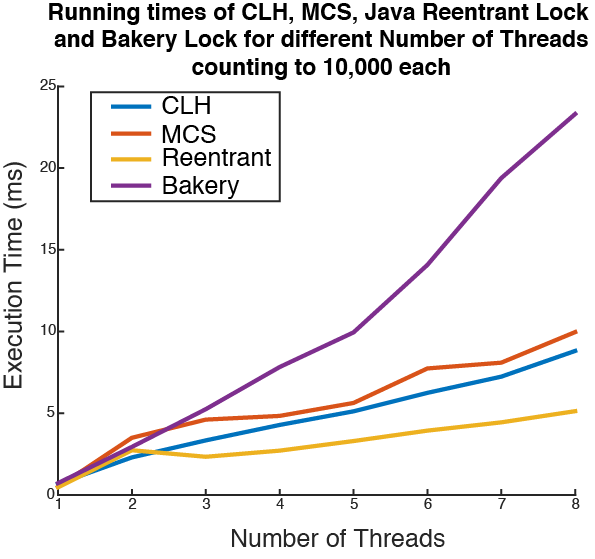
\includegraphics[scale = 1.1]{runningTime.png}
	\caption{Results of different locks and concurrent counting}\label{fig:counting}
\end{figure}

These results were found by averaging the execution of 500 trials for each case.  The results show that even between 1-8 threads, the execution time difference is already significantly separating between the locks.  We see that the Bakery Lock's execution time increases much faster than the other locks.  The CLH and the MCS are both comparable in speed, with CLH lock consistently being $\sim1$ millisecond faster.  The Java Reentrant Lock also stays consistently faster than the rest of the locks.

The test was only executed up to 8 threads because this is the number of cores on the test machine.  Once we pass the number of cores on the machine, the computer starts to create virtual threads, and these cause execution time to substantially increase.  Increasing the threads from 8 to 9 increased the execution time almost 10 fold.  Tests will be done to see if the execution time keeps its trend while executing with virtual threads, and with different computers with different processors.  However, we can still see the general trend of execution time and thread number using only up to 8 threads.  

\subsection*{\textsc{Difficulties}}
When implementing these locking algorithms, many bugs were encountered.  Both the CLH and MCS locks use a Queue for their implementation.  This queue is consisted of a "QNode" class; within this QNode class, the variables were initially declared as normal integers and normal references to next.  We found that this caused data racing to occur or false references to nodes.  These variables were changed to be atomic integers and atomic references.  Using atomic variables types helped stop data racing and thread failures.
\end{document}